\documentclass[portuguese,]{article}
\usepackage{lmodern}
\usepackage{amssymb,amsmath}
\usepackage{ifxetex,ifluatex}
\usepackage{fixltx2e} % provides \textsubscript
\ifnum 0\ifxetex 1\fi\ifluatex 1\fi=0 % if pdftex
  \usepackage[T1]{fontenc}
  \usepackage[utf8]{inputenc}
\else % if luatex or xelatex
  \ifxetex
    \usepackage{mathspec}
  \else
    \usepackage{fontspec}
  \fi
  \defaultfontfeatures{Ligatures=TeX,Scale=MatchLowercase}
\fi
% use upquote if available, for straight quotes in verbatim environments
\IfFileExists{upquote.sty}{\usepackage{upquote}}{}
% use microtype if available
\IfFileExists{microtype.sty}{%
\usepackage{microtype}
\UseMicrotypeSet[protrusion]{basicmath} % disable protrusion for tt fonts
}{}
\usepackage[margin=1in]{geometry}
\usepackage{hyperref}
\hypersetup{unicode=true,
            pdftitle={Exportações de Soja mesmo triturada},
            pdfauthor={Paulo Alencar},
            pdfborder={0 0 0},
            breaklinks=true}
\urlstyle{same}  % don't use monospace font for urls
\ifnum 0\ifxetex 1\fi\ifluatex 1\fi=0 % if pdftex
  \usepackage[shorthands=off,main=portuguese]{babel}
\else
  \usepackage{polyglossia}
  \setmainlanguage[]{portuguese}
\fi
\usepackage{graphicx,grffile}
\makeatletter
\def\maxwidth{\ifdim\Gin@nat@width>\linewidth\linewidth\else\Gin@nat@width\fi}
\def\maxheight{\ifdim\Gin@nat@height>\textheight\textheight\else\Gin@nat@height\fi}
\makeatother
% Scale images if necessary, so that they will not overflow the page
% margins by default, and it is still possible to overwrite the defaults
% using explicit options in \includegraphics[width, height, ...]{}
\setkeys{Gin}{width=\maxwidth,height=\maxheight,keepaspectratio}
\IfFileExists{parskip.sty}{%
\usepackage{parskip}
}{% else
\setlength{\parindent}{0pt}
\setlength{\parskip}{6pt plus 2pt minus 1pt}
}
\setlength{\emergencystretch}{3em}  % prevent overfull lines
\providecommand{\tightlist}{%
  \setlength{\itemsep}{0pt}\setlength{\parskip}{0pt}}
\setcounter{secnumdepth}{5}
% Redefines (sub)paragraphs to behave more like sections
\ifx\paragraph\undefined\else
\let\oldparagraph\paragraph
\renewcommand{\paragraph}[1]{\oldparagraph{#1}\mbox{}}
\fi
\ifx\subparagraph\undefined\else
\let\oldsubparagraph\subparagraph
\renewcommand{\subparagraph}[1]{\oldsubparagraph{#1}\mbox{}}
\fi

%%% Use protect on footnotes to avoid problems with footnotes in titles
\let\rmarkdownfootnote\footnote%
\def\footnote{\protect\rmarkdownfootnote}

%%% Change title format to be more compact
\usepackage{titling}

% Create subtitle command for use in maketitle
\newcommand{\subtitle}[1]{
  \posttitle{
    \begin{center}\large#1\end{center}
    }
}

\setlength{\droptitle}{-2em}
  \title{Exportações de Soja mesmo triturada}
  \pretitle{\vspace{\droptitle}\centering\huge}
  \posttitle{\par}
  \author{Paulo Alencar}
  \preauthor{\centering\large\emph}
  \postauthor{\par}
  \predate{\centering\large\emph}
  \postdate{\par}
  \date{5 de novembro de 2016}

\usepackage{booktabs}
\usepackage{longtable}
\usepackage{floatrow}
\usepackage[document]{ragged2e}

\floatsetup[figure]{capposition=top}
\floatsetup[table]{capposition=top}

\makeatletter
\setlength{\@fptop}{0pt}
\makeatother

\newcommand{\source}[1]{{
	\begin{flushleft}
		 \scriptsize{Fonte: {#1}}
	\end{flushleft}
 }}

\begin{document}
\maketitle

\section{Dados}\label{dados}

Os dados desse exemplo foram extraídos das séries históricas disponíveis
no site do \href{www.mdic.gov.br}{MDIC}.

Amostra dos dados:

\begin{table}[ht]
\centering
\caption{Amostra de dados} 
\begin{tabular}{crrr}
  \hline
DATA & VL\_FOB & KG\_LIQUIDO & PRECO \\ 
  \hline
Jan/1997 &     4.118.740 &     14.030.000 & 0,29 \\ 
  Fev/1997 &     4.896.148 &     17.095.000 & 0,29 \\ 
  Mar/1997 &   156.200.973 &    550.157.554 & 0,28 \\ 
  Abr/1997 &   462.887.400 &  1.598.886.449 & 0,29 \\ 
  Mai/1997 &   504.098.587 &  1.697.312.680 & 0,30 \\ 
  Jun/1997 &   395.752.981 &  1.345.808.797 & 0,29 \\ 
  Jul/1997 &   494.893.812 &  1.670.251.481 & 0,30 \\ 
  Ago/1997 &   291.057.057 &    986.597.810 & 0,30 \\ 
  Set/1997 &   104.112.390 &    348.746.010 & 0,30 \\ 
  Out/1997 &    32.397.210 &    105.540.943 & 0,31 \\ 
   \hline \multicolumn{1}{l}{\scriptsize{Fonte: MDIC}} \\\end{tabular}
\end{table}

A figura \ref{fig:fig1} apresenta a evolução do valor exportado de Soja
mesmo triturada. O recorde de valor aconteceu em maio de 2013, sendo
exportado o total de \textbf{US\$ 4.152.649.753}.

\begin{figure}[H]
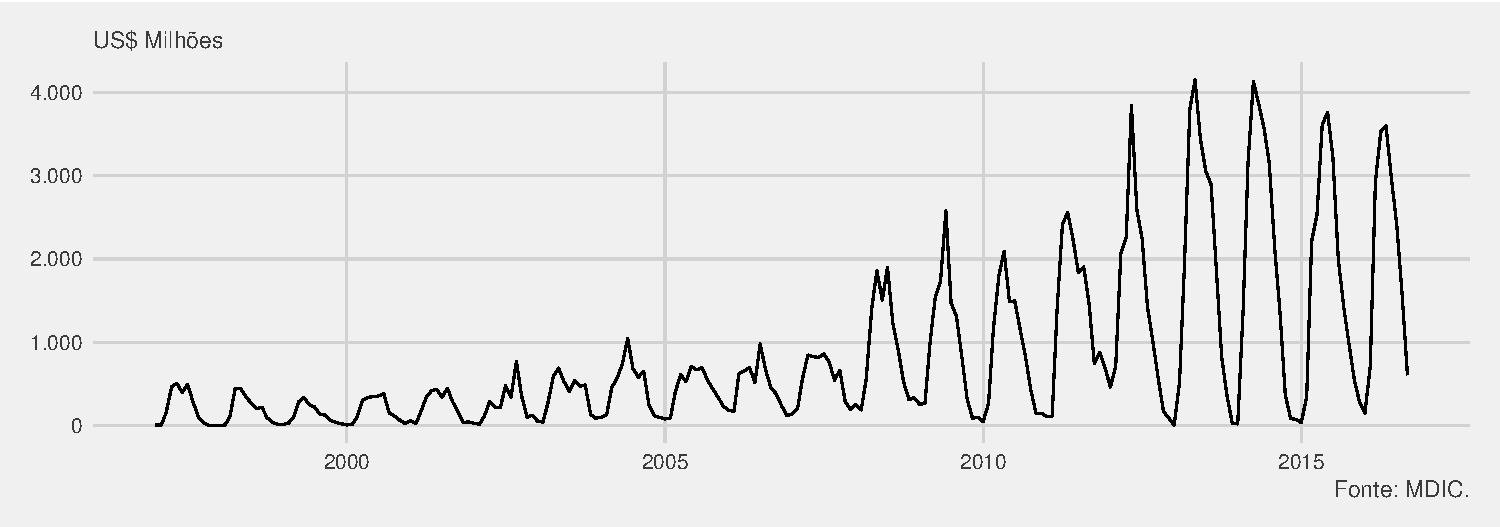
\includegraphics{exemplo_pdf_files/figure-latex/fig1-1} \caption{Valor Exportado de Soja mesmo triturada}\label{fig:fig1}
\end{figure}

Em relação ao volume exportado, o recorde ocorreu em abril de 2016, com
exportação de \textbf{10.075.226 toneladas}. A figura \ref{fig:fig2}
traz a evolução dessa variável.

\begin{figure}[H]
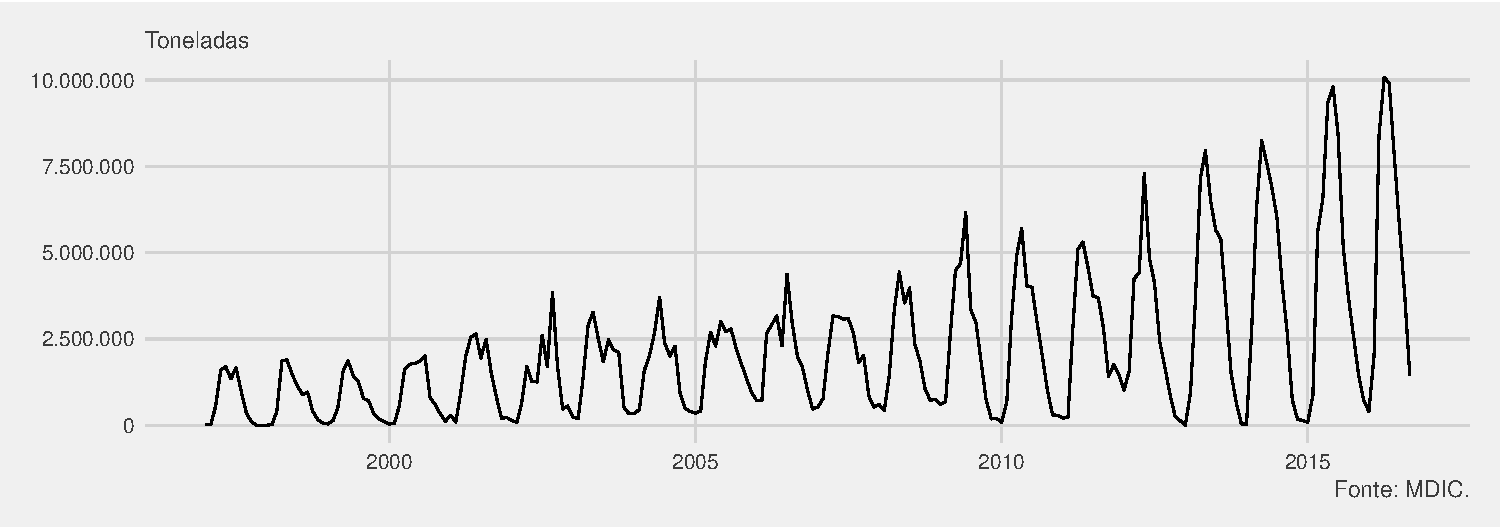
\includegraphics{exemplo_pdf_files/figure-latex/fig2-1} \caption{Volume Exportado de Soja mesmo triturada}\label{fig:fig2}
\end{figure}

O recorde de preço (US\$/KG) ocorreu em janeiro de 2013, chegando a
\textbf{US\$ 905,31} por \textbf{tonelada} exportada. A figura
\ref{fig:fig3} apresenta a série de preços.

\begin{figure}[H]
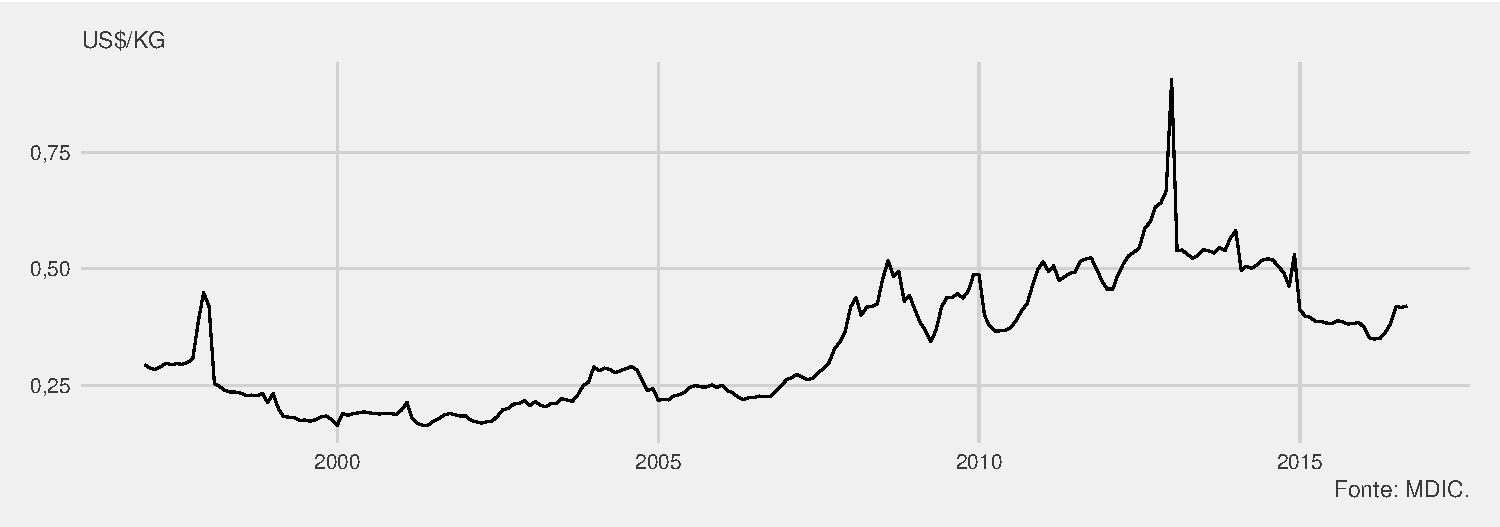
\includegraphics{exemplo_pdf_files/figure-latex/fig3-1} \caption{Preço Soja mesmo triturada}\label{fig:fig3}
\end{figure}

\subsection{Investigando a existência de
sazonalidade}\label{investigando-a-existencia-de-sazonalidade}

A figura \ref{fig:fig4} pode ser utilizada para avaliar a possível
presença de sazonalidade na série de volume de exportações de soja mesmo
triturada, Para cada mês é exibida a evolução do volume dentro do mês
(linha preta) e a média daquela mês (linha azul).

\begin{figure}[H]
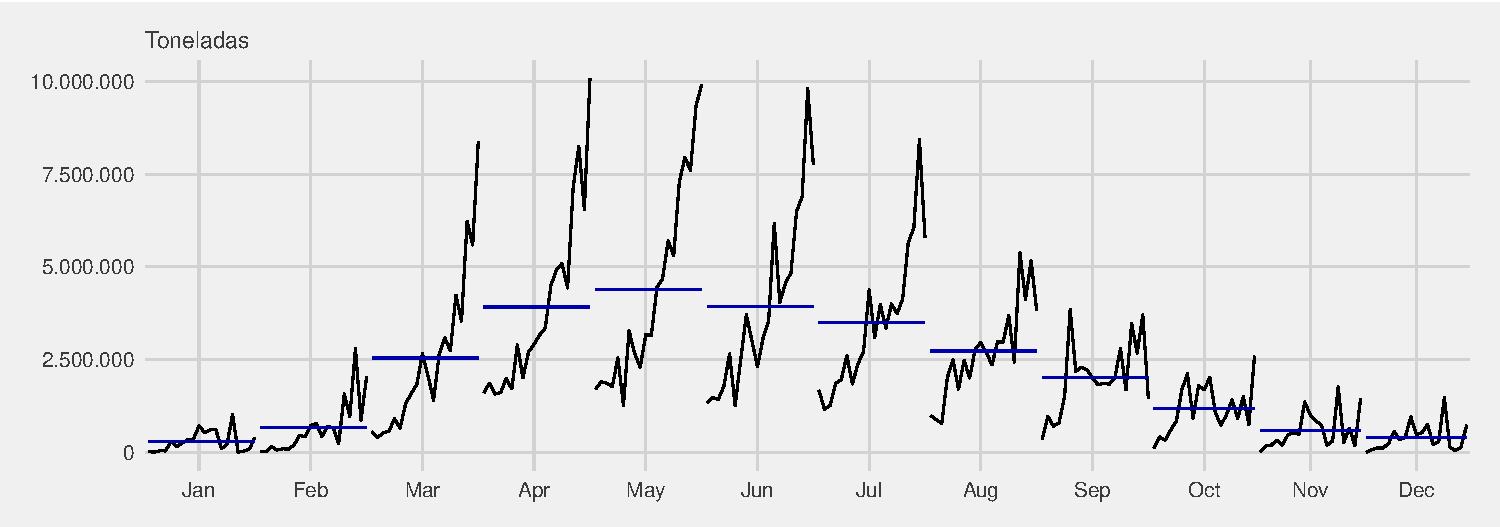
\includegraphics{exemplo_pdf_files/figure-latex/fig4-1}
\caption{Comparação Mensal dos Volumes Exportados}\label{fig:fig4}
\source{MDIC.}
\end{figure}


\end{document}
